\section{Design}

\subsection{UNO compontents}

My solution will be a LibreOffice extension that registers an UNO\cite{uno}
component. UNO is the interface based component model of LibreOffice. The main
feature it provides is that interfaces are defined in a language-idependent
IDL-like language, and they can be implemented in multiple languages:

\begin{itemize}
\item C
\item C++
\item Python
\item Java
\item BASIC
\end{itemize}

The caller is not aware which language the implementation uses, and it does not
need to, either. In my extension, I call BASIC macros from the menu elements,
which invoke the underlying Java code, where the business logic is implemented.

All the Java code is contained by a single jar file, the workflow of creating
it is the following:

\begin{figure}[H]
\centering
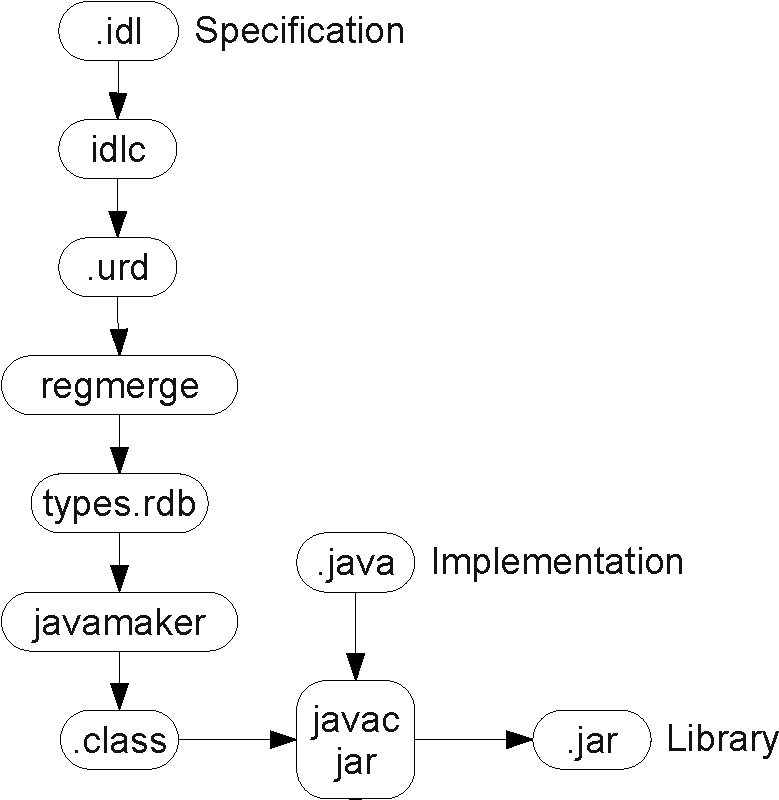
\includegraphics[width=250px,keepaspectratio]{uno-java.pdf}
\caption{Workflow of implementing an UNO service in Java}
\end{figure}

\begin{itemize}
\item \emph{idlc} compiles the .idl files to UNO Resource Descriptors,
\item \emph{regmerge} merges all the .urd files of the component to a single Resource Database,
\item \emph{javamaker} creates interfaces (.class files) from the Resource Database,
\item finally the standard Java development tools (\emph{javac}, \emph{jar})
creates the final jar, including the Java implementation.
\end{itemize}

Once the jar package is ready, a zip archive is created, containing:

\begin{itemize}
\item \emph{Addons.xcu}, containing the menu items
\item the BASIC library (callbacks for the menu items)
\item Java libraries used by the Java implementation
\item the Java implementation
\item metamodel of the stored settings
\item other files: metadata, extension description, license, etc.
\end{itemize}

Now that we saw the concept of UNO components and the structure of an
extension, the rest of this section describes the design of the UNO
specifications and Java implementations provided by the extension.

\subsection{The SharePoint library}

The Java implementation is split to two parts, the SharePoint library and the
user interface. The previous lives under the \emph{hu.vmiklos.lpsp} namespace,
the other does so under \emph{fr.starxpert.opal}.

The following UML package diagram shows these packages with their dependencies:

\begin{figure}[H]
\centering
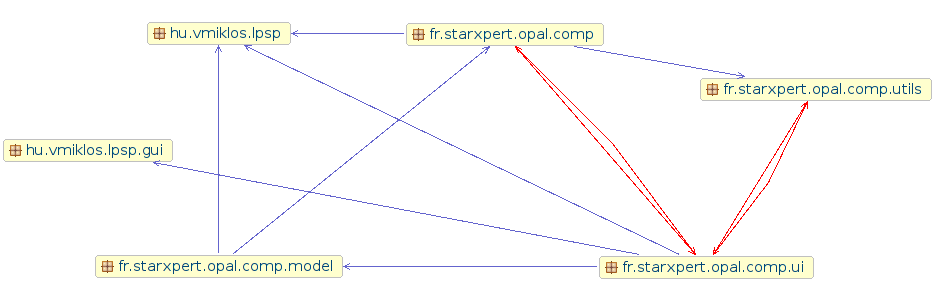
\includegraphics[width=425px,keepaspectratio]{design-packages.png}
\caption{Packages of the SharePoint extension}
\end{figure}

At the time of writing, there is no ready to use Java library to communicate
with a SharePoint server. Because of this, I decided to separate the SharePoint
protocol implementation from the LibreOffice-specific part of the extension to
make it reusable in other projects. It provides the following classes:

\begin{itemize}
\item \emph{Handler}: Handles requests from a frontend. Unless a feature has a
specific class, it is implemented here.
\item \emph{PacketParser}: Extracts the error message from a Vermeer
RPC\cite{vermeer} response packet.
\item \emph{FileOpenRootParser}: Parses the result from the \emph{list
workspaces} request.
\item \emph{FileOpenParser}: Parses the result from the \emph{list directory of
a workspace} request.
\item \emph{LastModParser}: Parses the result from the \emph{get last
modification date} request.
\item \emph{Version}: Handles document versions.
\item \emph{Messages}: Provides localization for the library error messages.
\item \emph{HandlerTest}: Automatically tests all features on a given server
using JUnit.
\end{itemize}

I paid attention in my solution to not require additional server-side component
installation, the SharePoint library can communicate with a standard SharePoint
server, without any server modifications.

\subsection{The UNO interfaces}

The UNO interfaces are reused from the already referenced OPAL (OpenOffice
Plugin for Alfresco) extension. Many of them contains the \emph{Alfresco} word,
referring to the underlying protocol. I did not change the interface name
(since they are not visible to the user), however of course I changed the
underlying implementation.

It's an UNO convention that interfaces start with a capital X. The following
interfaces are provided by the extension:

\begin{itemize}
\item \emph{XAlfrescoFilePicker}: an open/save as file picker.
\item \emph{XAlfrescoVersions}: a versions dialog.
\item \emph{XAlfrescoDocument}: a document received from the
SharePoint server.
\item \emph{XAlfrescoDocumentManager}: a storage for XAlfrescoDocument instances.
\item \emph{XAuthenticationManager}: a handler for different authentication mechanisms.
\item \emph{XConnection}: a connection to a SharePoint server.
\end{itemize}

The extension provides a single exception type -- \emph{AlfrescoException} --
when it throws errors.

It also provides a single enumeration type -- \emph{FileTypes} -- to declare
the list of LibreOffice applications it handles. (It's current value is:
Writer, Calc, Impress and Draw.)

UNO services are interfaces containing static methods only.  The following
services are provided by the extension:

\begin{itemize}
\item \emph{AlfrescoDocument}: factory for XAlfrescoDocument.
\item \emph{Connection}: implementation for XConnection.
\item \emph{theAlfrescoDocumentManager}: singleton for XAlfrescoDocumentManager.
\item \emph{theAuthenticationManager}: singleton for XAuthenticationManager.
\item \emph{AlfrescoFilePicker}: implementation for XAlfrescoFilePicker.
\item \emph{AlfrescoVersions}: implementation for XAlfrescoVersions.
\end{itemize}

\subsection{User interface}

The user interface lives in the \emph{ft.starxpert.opal.comp} package, based on
the original OPAL extension. The classes of the user interface are organized in
4 Java packages:

\begin{itemize}
\item \emph{ft.starxpert.opal.comp.model}: a model for the folder and document
structure, used by the file pickers (\emph{open} and \emph{save as} dialog
windows).
\item \emph{ft.starxpert.opal.comp.ui}: contains the dialog classes.
\item \emph{ft.starxpert.opal.comp.util}: miscellaneous utility classes for UNO and localization.
\item \emph{ft.starxpert.opal.comp}: classes implementing the rest of UNO
services: authentication manager, document manager, document, connection, etc.
\end{itemize}

The user interface dialogs are reachable from the \emph{Document repository}
menu item, which is registered by the \emph{Addons.xcu} configuration file,
which is a standard configuration file of LibreOffice extensions.

The following menu items are designed:

\begin{itemize}
\item Connection: force connecting to an other document management server, even
if the user is already connected.
\item Open: downloads an existing document from the server.
\item Close: discards the local copy of a downloaded document.
\item Save: save the document model and upload the saved local copy to the server.
\item Save as: upload the local document to the server using a new name.
\item Versions: management of document versions.
\end{itemize}

The menu items call BASIC macros, which invoke UNO services. Those services are
finally implemented in the Java user interface.

The macros are split into two packages: the ones directly called by the menu
items, and the other utility macros.

The menu items call the following macros (\emph{OPAL.menu} package):

\begin{itemize}
\item getConnection: shows the Connection dialog.
\item openFile: shows the File Open dialog.
\item closeFile: closes the current document via the document manager, the
already registered close listener will handle the cleanup of the local document
copy.
\item saveFile: saves the document via the document manager.
\item saveAsFile: shows the Save As dialog.
\item openVersion: shows the dialog listing versions of the document.
\end{itemize}

The following ones are the utility macros (\emph{OPAL.utils} package):

\begin{itemize}
\item getDocumentManager: returns the document manager singleton.
\item getAuthenticationManager: returns the document manager singleton.
\item getCurrentAlfrescoDocument: asks the document model of the current LibreOffice component (Writer document, Calc spreadsheet, etc.) from the document manager.
\item getCurrentConnection: asks the current connection from the authentication manager.
\end{itemize}

The BASIC macros invoke the following UNO Services:

\begin{itemize}
\item Connection: calls \emph{theAuthenticationManager::execute()}.
\item Open: calls \emph{AlfrescoFilePicker::execute()} with \emph{IsOpen = true}.
\item Close: calls \emph{theAlfrescoDocumentManager::getAlfrescoDocument()}, \\ then the \emph{close} method on the returned result.
\item Save: calls \emph{theAlfrescoDocumentManager::getAlfrescoDocument()}, \\ then the \emph{save} method on the returned result.
\item Save as: calls \emph{AlfrescoFilePicker::execute()} with \emph{IsOpen = false}.
\item Versions: calls \emph{AlfrescoVersions::execute()}
\end{itemize}

At this point, we know the user interface entry points in our Java
implementation. As mentioned above, Java bytecode for the UNO services are
automatically generated (by \emph{javamaker}). Now one may ask: how does the
stub know where is the real implementation? This is handled by the
\emph{RegistrationHandler} class. The list of implementation classes
implementing a UNO service is in the \emph{RegistrationHandler.classes} file.
Each implementation class specifies what service does it implement, then the
registration handler collects this information and returns to UNO, when it is
asked. Finally, the \emph{RegistrationClassName:} header in the
\emph{META-INF/MANIFEST.MF} file of the Jar package defines the registration
handler class name.

As a result, the following entry points are designed in the Java
implementation:

\begin{itemize}
\item Connection: \emph{AuthenticationManagerImpl.execute()}
\item Open: \emph{AlfrescoFilePickerImpl.execute()}
\item Close: \emph{AlfrescoDocumentManagerImpl.getAlfrescoDocument()}, \\ then \emph{AlfrescoDocumentImpl.close()}
\item Save: \emph{AlfrescoDocumentManagerImpl.getAlfrescoDocument()}, \\ then \emph{AlfrescoDocumentImpl.save()}
\item Save as: \emph{AlfrescoFilePickerImpl.execute()}
\item Versions: \emph{AlfrescoVersionsImpl.execute()}
\end{itemize}

These classes contain all the business logic and they call the SharePoint
library for communication. The dialog windows are separated from UNO
interfaces, they are always implemented in separate classes. Given that there
are common tasks for all of our user interface dialogs, there is a common
ancestor for all of them, called \emph{AbstractDialog}.

The following dialog classes are included in the \emph{ui} package:

\begin{itemize}
\item Connection: \emph{ConnectionDialog} (connect dialog), \\
\emph{ConfigServerDialog} (server list), \\ \emph{ServerDialog} (settings for an
individual target)
\item Open, save as: \emph{FilePickerDialog}
\item Close: None.
\item Save: \emph{CommentVersionDialog}
\item Versions: \emph{VersionsDialog}
\end{itemize}

An UML class diagram showing these classes is available on the next page.

\begin{figure}[p]
\centering
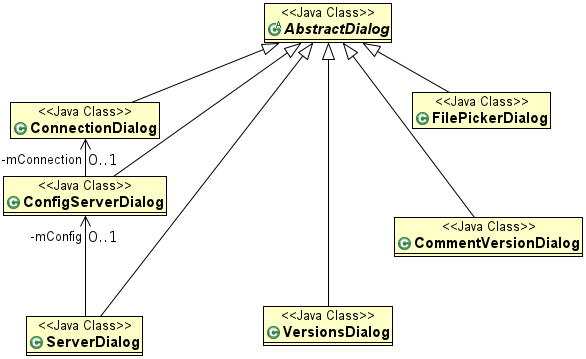
\includegraphics[width=400px,keepaspectratio]{design-spui.png}
\caption{Classes of the user interface}
\end{figure}
